\newpage
\pagestyle{empty}

\begin{minipage}[c]{.25\linewidth}
	\includegraphics[width=4cm]{images/Logo-LEnsE.png}
\end{minipage} \hfill
\begin{minipage}[c]{.4\linewidth}

\begin{center}
\vspace{0.3cm}
{\Large \textsc{Opto-Électronique}}

\medskip

\textbf{\Large Ressources}

\end{center}
\end{minipage}\hfill

\vspace{0.5cm}

\noindent \rule{\linewidth}{1pt}
\section{Tracer la caractéristique statique d'un dipôle}
\label{ressource:CaracStat}


%%%%%%%%%%%%%%%%%%%%%%%%%%%%%%%%%%%%%%%%%%%%%%%%%%%%%%%%%%%%%%%%%%%%%%%%%%%%%%%%
%%%%%

En électronique, la caractéristique statique d'un dipôle correspond à la relation mathématique $i=f(u)$ qu'il existe entre la différence de potentiel $u$ à ses bornes et le courant $i$ le traversant, dans des conditions statiques, c'est-à-dire lorsque ces deux grandeurs ne sont pas dépendantes du temps.

\medskip

Il existe deux méthodes principales pour caractériser statiquement un dipôle :

\begin{itemize}
	\item \textbf{une méthode manuelle}, qui permet de tracer point à point cette courbe, en faisant varier $u$ aux bornes du dipôle et en mesurant $u$ et $i$ pour un certain nombre de points,
	\item \textbf{une méthode automatique}, qui permet d'obtenir de manière plus rapide une allure de la caractéristique statique sur un oscilloscope.
\end{itemize}

\bigskip

\subsection{Exemple de résultats}

La figure~\ref{fig:carac_led} présente un exemple de résultats obtenus pour une LED jaune classique (5 mm).

La caractéristique manuelle a été tracée à l'aide d'un multimètre \textit{Fluke 45} (en mode DC pour mesurer le courant et la tension) et en insérant une résistance $R_P$ de $150\operatorname{\Omega}$ (voir circuit de mesure en figure~\ref{fig:carac_led_man}).

La caractéristique automatique a été mesurée à l'aide d'un oscilloscope \textit{Voltcraft DSO1084F}. Une résistance de protection $R_P$ de $150\operatorname{\Omega}$ a été choisie ainsi qu'une résistance $R_I$ de $10\operatorname{\Omega}$ (voir circuit de mesure en figure~\ref{fig:carac_led_auto}). Un signal triangulaire de fréquence de $10\operatorname{Hz}$ et d'amplitude crête à crête de $5\operatorname{V}$ a été appliqué sur l'ensemble du circuit. 



\begin{figure}[h!]
    \centering
	\includegraphics[width=0.9\textwidth]{images/caract_led_phd.png}

    \caption{Résultats de mesure de la caractéristique statique d'une LED jaune. Tableau et courbe otenus par la méthode manuelle (à gauche). Capture d'écran d'oscilloscope obtenue par la méthode automatique (calibre de 1V/carreau en horizontal et de 100mV/carreau en vertical).}
    \label{fig:carac_led}
\end{figure}

\newpage
\section{Caractéristique Manuelle}

Une première méthode pour pouvoir \textbf{tracer la caractéristique statique} $i=f(u)$ d'un dipôle est de faire varier la différence de potentiel à ses bornes de manière statique (i.e. très lente) et de mesurer la différence de potentiel $u$ aux bornes du dipôle, à l'aide d'un voltmètre, et le courant $i$ le traversant, à l'aide d'un ampèremètre, point par point.

\medskip

Pour \textbf{faire varier la différence de potentiel} aux bornes du dipôle, on pourra prendre une \textbf{alimentation stabilisée réglable}.

Pour \textbf{mesurer la différence de potentiel} aux bornes du dipôle, on pourra utiliser un multimètre en mode \textbf{voltmètre} câblé en parallèle du dipôle.

Pour \textbf{mesurer le courant} traversant le dipôle, on pourra utiliser un multimètre en mode \textbf{ampèremètre} câblé en série avec le dipôle.

\subsection{Circuit de mesure}

On donne le schéma de la figure~\ref{fig:carac_led_man} pour mesurer à la fois le courant et la différence de potentiel aux bornes d'un dipôle (ici une LED).

\bigskip

\begin{figure}[h!]
    \centering
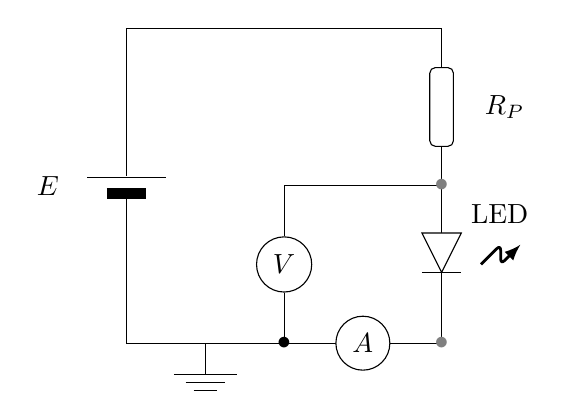
\begin{tikzpicture}
    \draw(0,-2)--(0,2)--(4,2)--(4,-2)--cycle;
    \node[fill=white, minimum height= 0.2cm] at (0,0) {}; 
    \draw(-0.5,0.1)--++(1,0);
    \draw[line width=4pt] (-0.25,-0.1)--++(0.5,0);
    
    
    %\draw[fill=white] (0,0) circle (0.5cm);
    %\draw [>=stealth, ->, very thick] (0,-0.25)--(0,0.25);
    \node at (-1,0) {$E$};
    \node[draw, fill=white, minimum width=0.3cm, minimum height=1cm, rounded corners =2pt] at (4,1) {};
    \node [xshift=0.8cm] at (4,1) {$R_{P}$};
    \draw(1,-2)--++(0,-0.4); \draw(0.6,-2.4)--++(0.8,0); \draw (0.75,-2.5)--++(0.5,0);\draw (0.85,-2.6)--++(0.3,0); 
    
    \node[circle,draw, fill =white](Voltmetre) at (2,-1) {$\operatorname{V}$};
    \draw (Voltmetre.north)|-(4,0) node[gray] {$\bullet$};
    \draw (Voltmetre.south)--(2,-2) node {$\bullet$};
    \node[circle,draw, fill =white](Ametre) at (3,-2) {$\operatorname{A}$};
    \node[gray] at (4,-2) {$\bullet$};

    %\draw (Ametre.east)--++(1,0) node (int) [midway]   {$\bullet$} --++(0,1) --++(0.4,0.8);
%\draw (0.5,2) -| (4.4,0.5);
%\draw (0.5,-1)  -|(Ametre.west);
%\draw (Voltmetre.north)--(2,2) node {$\bullet$};
%\draw (Voltmetre.south)--(2,-1) node {$\bullet$};

    
            \begin{scope}[xshift=3.75cm,yshift=-0.6cm]%LED
            \draw[fill=white] (0,0)--++(0.5,0)--++(-0.25,-0.5)--cycle;
            \draw (0,-0.5)--++(0.5,0) node[above right, yshift=0.5cm]{LED};
            \draw[->,>=latex,rounded corners=2pt, line width=1pt] (0.75,-0.4) --++ (0.25,0.25)--++(0,-0.25)--++(0.25,0.25);
            \node (A1) at (0.25,0) {};
            \node (K1) at (0.25,-0.5) {};
            \end{scope}        
\end{tikzpicture}
    \caption{Schéma du circuit de mesure de la caractéristique statique par la méthode manuelle. Le dipôle à caractériser est ici représenté par une LED. La résistance $R_P$ est une résistance de protection permettant de limiter le courant dans le dipôle à caractériser.}
    \label{fig:carac_led_man}
\end{figure}



\subsection{Méthode de mesure}

On mesure à la fois le courant, à l'aide de l'ampèremètre branché en série, et la différence de potentiel aux bornes de la LED, à l'aide d'un voltmètre branché en parallèle.

On fait alors varier le potentiel de la source de tension $E$, pour relever, pour plusieurs points, les valeurs du courant (A) et de la différence de potentiel (V).

La plupart des multimètres permettent d'afficher simultanément la tension et le courant continu.

Les points peuvent ensuite être enregistrés dans un fichier de tableur (type Excel ou Calc). Cet outil logiciel permettra par la suite de tracer la courbe $i=f(u)$.



\newpage
\section{Caractéristique Automatisée}

Une seconde méthode permettant d'\textbf{obtenir une allure de la caractéristique statique }$i=f(u)$ d'un dipôle est de faire varier la différence de potentiel à ses bornes en appliquant un signal dont l'amplitude varie lentement dans le temps. On peut alors mesurer la différence de potentiel $u$ aux bornes du dipôle et le courant $i$ le traversant à l'aide d'un oscilloscope en mode XY.

Cette méthode va nécessiter de \textbf{transformer le courant en différence de potentiel}, seule grandeur mesurable à l'aide d'un oscilloscope.

Pour faire \textbf{varier la différence de potentiel} aux bornes du dipôle, on utilisera une \textbf{générateur basse fréquence} (ou GBF).

Pour \textbf{mesurer la différence de potentiel} aux bornes du dipôle, on pourra utiliser une des voies de l'\textbf{oscilloscope} câblée en parallèle du dipôle.

Pour \textbf{mesurer le courant} traversant le dipôle, on insérera une \textbf{résistance de faible valeur} (afin de ne pas perturber le reste du montage par l'ajout d'un système de mesure) en série avec le dipôle que l'on cherche à caractériser. On pourra alors utiliser la seconde voie de l'\textbf{oscilloscope} pour mesurer la différence de potentiel aux bornes de cette résistance. Par la loi d'Ohms, on retrouvera alors la valeur du courant.

\subsection{Circuit de mesure}

On donne le circuit de la figure~\ref{fig:carac_led_auto} pour tracer de manière automatisée l'allure de la caractéristique statique.

La résistance $R_P$ est une résistance de protection du dipôle à caractériser (ici une LED).

La résistance $R_I$ permet de convertir le courant traversant la branche en différence de potentiel mesurable par l'oscilloscope.


\begin{figure}[h!]
    \centering
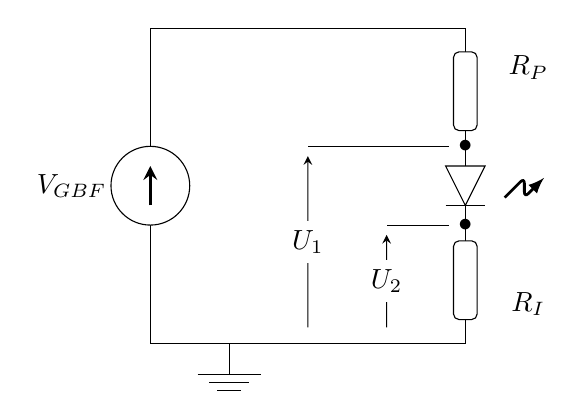
\begin{tikzpicture}
    \draw(0,-2)--(0,2)--(4,2)--(4,-2)--cycle;
    \draw[fill=white] (0,0) circle (0.5cm);
    \draw [>=stealth, ->, very thick] (0,-0.25)--(0,0.25);
    \node at (-1,0) {$V_{\text{GBF}}$};
    \node[draw, fill=white, minimum width=0.3cm, minimum height=1cm, rounded corners =2pt] at (4,1.2) {};
    \node [xshift=0.8cm] at (4,1.5) {$R_{P}$};
    \draw(1,-2)--++(0,-0.4); \draw(0.6,-2.4)--++(0.8,0); \draw (0.75,-2.5)--++(0.5,0);\draw (0.85,-2.6)--++(0.3,0); 
     \node[draw, fill=white, minimum width=0.3cm, minimum height=1cm, rounded corners =2pt] at (4,-1.2) {};
    \node [xshift=0.8cm] at (4,-1.5) {$R_I$};
            \begin{scope}[xshift=3.75cm, yshift=0.25 cm]%LED
            \draw[fill=white] (0,0)--++(0.5,0)--++(-0.25,-0.5)--cycle;
            \draw (0,-0.5)--++(0.5,0); %node[above right, yshift=0.5cm]{LED};
            \draw[->,>=latex,rounded corners=2pt, line width=1pt] (0.75,-0.4) --++ (0.25,0.25)--++(0,-0.25)--++(0.25,0.25);
            \node (A1) at (0.25,0) {};
            \node (K1) at (0.25,-0.5) {};
            \end{scope}        
            
           \node[yshift=0.25 cm]  (CH1) at (A1){$\bullet$};
            \node[yshift=-0.25 cm] (CH2)   at (K1){$\bullet$};
           \draw (CH1) --++(-2,0) node (VCH1) {};
           \draw (CH2) --++(-1,0)node (VCH2) {};
%            
           \draw [<-, >=stealth] (VCH1) -- (2,-1.8) node [midway, fill=white] {$U_{1}$};
            \draw [<-, >=stealth] (VCH2) -- (3,-1.8) node [midway, fill=white] {$U_{2}$};
\end{tikzpicture}
    \caption{Schéma du circuit de mesure de la caractéristique statique par la méthode automatique. Le dipôle à caractériser est ici représenté par une LED. La résistance $R_P$ est une résistance de protection permettant de limiter le courant dans le dipôle à caractériser. La résistance $R_I$ permet de convertir le courant en une tension mesurable à l'oscilloscope.}
    \label{fig:carac_led_auto}
\end{figure}


	
\newpage	
\subsection{Méthode de mesure}

On applique un signal dont l'amplitude varie dans le temps à l'aide du GBF : un signal triangulaire par exemple à une fréquence de quelques Hertz. \textit{On s'assurera que l'amplitude du signal fourni par le GBF est inférieure aux limitations des composants du montage.}

En mesurant à l'oscilloscope les tensions $U_1$ sur une voie et $U_2$ sur l'autre voie, on accède à une image de la tension aux bornes du dipôle  $U_1 - U_2$ (assimilable à $U_1$ si $U_2$ est faible pour toutes les valeurs de $i$) et à une image du courant traversant $R_I$ ($U_2$).

En traçant alors $U_2$ en fonction de $U_1$ (mode XY de l'oscilloscope), l'allure de la caractéristique statique du dipôle s'affiche alors.

\medskip

La figure~\ref{fig:carac_led_auto_res} montre le résultat d'une acquisition à l'oscilloscope des signaux $U_1$, $U2$ et $V_{GBF}$ obtenu lors de la mesure de la caractéristique d'une LED jaune classique (5 mm) à l'aide de résistances $R_P = 150\operatorname{\Omega}$ et $R_I = 10\operatorname{\Omega}$.

\begin{figure}[h!]
    \centering
	\includegraphics[width=0.9\textwidth]{images/carac_phd_time_xy.png}
	
	
    \caption{Évolution de la tension d'entrée (voie 4 en haut), de la tension $U_1$ aux bornes de l'ensemble LED et résistance $R_I$ (signal bleu - voie 1) et de la tension $U_2$ aux bornes de $R_I$ (image du courant - signal rouge - voie 2). Calibre de 1V/carreau pour $U_1$, de 50mV/carreau pour $U_2$ et de 2V/carreau pour $V_{GBF}$.}
    \label{fig:carac_led_auto_res}
\end{figure}



\subsection{Choix de $R_I$}

On cherche à mesurer $U_2$ (image du courant traversant le dipôle à caractériser) en fonction de $U_1 - U_2$ (tension aux bornes du dipôle à caractériser).

A l'aide de l'oscilloscope, sans sonde différentielle, il n'est pas possible de mesurer $U_1 - U_2$ directement et de l'affecter à son mode XY. Il sera donc uniquement possible de tracer $U_2$ en fonction de $U_1$. 

Pour que $U_1 - U_2$ soit assimilable à $U_1$ il faut que $U_2$ soit négligeable par rapport à $U_1$. En choisissant $R_I$ très faible on peut négliger $U_2$ par rapport à $U_1$ (sur une certaine gamme de courant).

\bigskip

\textit{Attention} : en prenant $R_I$ trop faible, on peut arriver à une tension non mesurable et donc non exploitable !
